  \begin{figure}
    \centering

    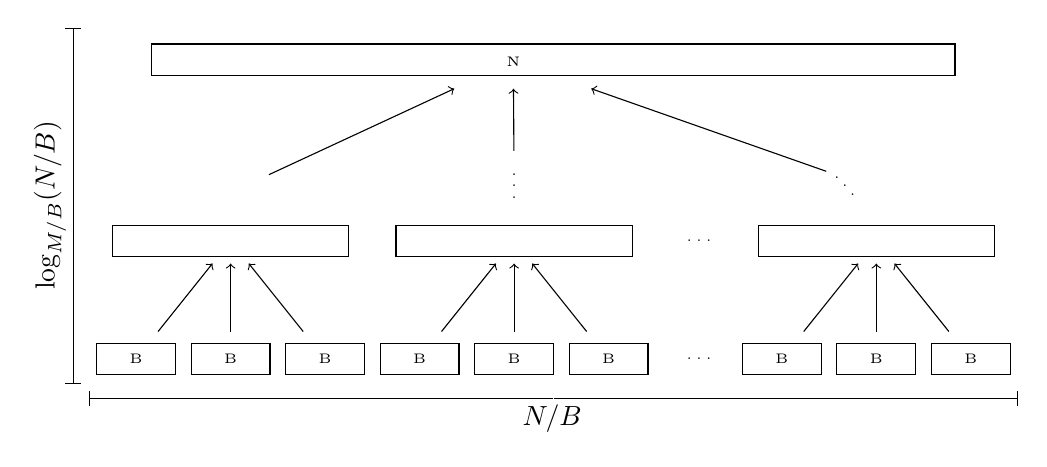
\begin{tikzpicture}
      % Base Case

      \tiny

      \onslide<2-> {
        \draw[] (0.0,0.0)  rectangle ++(1,0.4) node[pos=.5, inner sep=8] (l1b1) {B};
      }
      \onslide<3-> {
        \draw[] (1.2,0.0)  rectangle ++(1,0.4) node[pos=.5, inner sep=8] (l1b2) {B};
      }
      \onslide<4-> {
        \draw[] (2.4,0.0)  rectangle ++(1,0.4) node[pos=.5, inner sep=8] (l1b3) {B};
      }
      \onslide<5-> {
        \draw[] (3.6,0.0)  rectangle ++(1,0.4) node[pos=.5, inner sep=8] (l1b4) {B};
      }
      \onslide<6-> {
        \draw[] (4.8,0.0)  rectangle ++(1,0.4) node[pos=.5, inner sep=8] (l1b5) {B};
      }
      \onslide<7-> {
        \draw[] (6.0,0.0)  rectangle ++(1,0.4) node[pos=.5, inner sep=8] (l1b6) {B};
      }
      \onslide<8-> {
        \node at (7.65,0.2) {$\dots$};
        \draw[] (8.2,0.0)  rectangle ++(1,0.4) node[pos=.5, inner sep=8] (l1b7) {B};
      }
      \onslide<9-> {
        \draw[] (9.4,0.0)  rectangle ++(1,0.4) node[pos=.5, inner sep=8] (l1b8) {B};
      }
      \onslide<10-> {
        \draw[] (10.6,0.0) rectangle ++(1,0.4) node[pos=.5, inner sep=8] (l1b9) {B};

        % HACK: For some reason, when doing this horisontally, we get an
        %       unwanted horizontal '|' at the beginning.
        \draw[-|] (5.7,-0.3) edge ++(-5.8,0.0);
        \draw[-|] (5.9,-0.3) edge node[pos=-0.-0.02, below] {\normalsize $N/B$} ++(5.8,0.0);
      }

      % Merge level

      \onslide<11-> {
        \draw[] (0.2,1.5) rectangle ++(3.0,0.4) node[pos=.5, inner sep=8] (l2b1) {};
        \draw[->]
          (l1b1) edge (l2b1)
          (l1b2) edge (l2b1)
          (l1b3) edge (l2b1)
        ;
      }

      \onslide<12-> {
        \draw[] (3.8,1.5) rectangle ++(3.0,0.4) node[pos=.5, inner sep=8] (l2b2) {};
        \draw[->]
          (l1b4) edge (l2b2)
          (l1b5) edge (l2b2)
          (l1b6) edge (l2b2)
        ;
      }

      \onslide<13-> {
        \node at (7.65,1.7) {$\dots$};

        \draw[] (8.4,1.5) rectangle ++(3.0,0.4) node[pos=.5, inner sep=8] (l2b3) {};
        \draw[->]
          (l1b7) edge (l2b3)
          (l1b8) edge (l2b3)
          (l1b9) edge (l2b3)
        ;
      }

      % Final Result
      \onslide<14-> {
        \node at (2.1,2.5) (dots1) {$\iddots$};
        \node at (5.3,2.5) (dots2) {$\vdots$};
        \node at (9.5,2.5) (dots3) {$\ddots$};

        \draw[] (0.7,3.8) rectangle ++(10.2,0.4) node[pos=.45, inner sep=8] (N)
          {\phantom{PHANTOM}N\phantom{PHANTOM}};

        \draw[->]
          (dots1) edge (N)
          (dots2) edge (N)
          (dots3) edge (N)
        ;
      }

      \onslide<15-> {
        % HACK: Again, we get the horizontal '|' at the beginning of the edge.
        \draw[-|] (-0.3,-0.1) edge
                    node[pos=0.5, left, rotate=90, above=] {\normalsize$\log_{M/B}(N/B)$}
                    ++(0,4.5)
                  ;
      }

    \end{tikzpicture}
  \end{figure}
